\documentclass[]{article}
\usepackage{graphicx}
\graphicspath{ {graphs/} }
\usepackage{geometry}
\usepackage{gensymb}
\usepackage{booktabs}

%opening
\title{Identification of DC Pixels using Boosted Decision Trees}
\author{Robert Stein}
\begin{document}

\maketitle

\begin{abstract}
A new method of Direct Cherenkov (DC) pixel identification, relying on machine learning, was developed. A set of Cosmic Ray telescope images for training were each simulated twice, both with and without the Extended Air Shower (EAS) background, enabling the DC pixel in every realistic telescope images to be reliably identified using the corresponding background-free image. Using all pixels from these realistic training images, a Boosted Decision Tree (BDT) was trained to identify DC pixels. The BDT performance was tested on a second set of test realistic telescope images, and compared to existing methods of DC pixel identification.  
\end{abstract}

\section{Introduction}
In Cosmic Ray air showers, the primary particle will often emit DC light in the upper atmosphere, before generating an EAS in interaction with the lower atmosphere. In telescope images, this DC light is usually concentrated in a single  \textquoteleft DC pixel'. Identifying this pixel is challenging, because the DC light is much fainter than that from the EAS, which will be recorded in the DC pixel and many of surrounding pixels. As a result, most telescope images will have many bright pixels adjacent to one another, among which one will be the DC pixel. However, if found, the DC pixel can indicate the primary particle energy and charge. 

Currently, the DC pixel is identified after applying a number of cuts first, used a method developed by the HESS collaboration \cite{hess07}. From the subset of events passing these cuts, the variable \[Q_{DC} = \frac{Intensity}{Intensity_{N.N.max}}\] is defined as the ratio of the intensity of a pixel to the largest neighbouring pixel intensity. The DC pixel candidate is simply that with the largest $Q_{DC}$ among those passing the cuts. However, this method is neither reliable nor efficient. An improved method would aim to increase the number of correctly identified events, and enable cuts which better discriminate between correctly and incorrectly identified events.

Using the CORSIKA package, Cosmic Ray events were simulated both with and without an EAS component. The sim\textunderscore telarray package was used to simulate the resultant telescope image, assuming the events were observed by the HESS telescope array. Using the EAS-free image to reliably identify the DC pixel, a Boosted Decision Tree (BDT) was trained on each pixel from a training set of telescope images. The pixel information was provided in the form of individual pixel entries, rather than as discrete sets for images or events.

Once trained, the BDT was applied to every pixel entry in a separate 'testing' set of simulated telescope images. For each pixel, the BDT assigned a \textquoteleft Signal Probability', $P_{signal}$, indicating the likelihood of the pixel being the DC pixel. From an entire image, the pixel with the largest $P_{signal}$ was identified as the DC pixel candidate. Repeating the double simulation technique for the test data, the true DC pixels in the test telescope images were reliably identified from EAS-free images. Thus, the accuracy of BDT identification for test telescope images was calculated.

\section{Image Simulation}
A full simulation of Cosmic Ray air showers was performed using the CORSIKA package \cite{Heck98}, assuming a standard atmospheric profile derived from measurements conducted at the HESS site in Namibia. The simulated particles were $Fe^{56}$, within the Energy Range of $35-135$ TeV and a spectrum $\phi \propto E^{-2.7}$. For each set of simulated event, 4 unique random number seeds were used to generate the shower. An altitude of 1800m was assumed, again corresponding to the HESS site. The simulated zenith angle ranged from $0\degree < \theta < 2 \degree$, while the simulated azimuth angle ranges from $-2\degree < \phi < 2 \degree$. The four smaller HESS-phase-1 telescopes were arranged in a cross along the x/y axis with the larger HESS-phase-2 \textquoteleft CT5' telescope placed at the center. The length of each cross arm was $85m$. The simulated target region of the cores was chosen to be a square centered on CT5, with each 300m-long side bisecting the x/y axis.

In order to identify the DC pixel, a simulation was initially run with an energy cut of 10 PeV on all muons and electrons. Because this cut exceeded the primary particle energy, neither daughter muons and electrons, nor the photons they would have emitted, were simulated. Thus the hadronic Cherenkov Light from the primary particle and daughter fragments, but not the EAS light, was present in the camera image. A second identical \textquoteleft EAS Simulation' was run including the same random seeds, but without the energy cut on muons and electrons. This gave a complete EAS image including the DC light.

Using the sim\textunderscore telarray package \cite{Bernlohr08}, the expected HESS hardware response to each air shower was simulated. Among other things, the program accounts for atmospheric transmission and density, mirror positions, sizes and reflectivities, camera shadowing and triggering, quantum efficiency and pulse responses. Due to the comprehensive and detailed nature of these hardware simulations, the resultant images can be considered \textquoteleft realistic camera images'. For the EAS Simulation, the night sky background was also included by sim\textunderscore telarray, further obscuring the DC pixel.

\begin{figure}
\newgeometry{a4paper, portrait, margin=1.0in}
\centering
\begin{minipage}{0.45\textwidth}
\centering
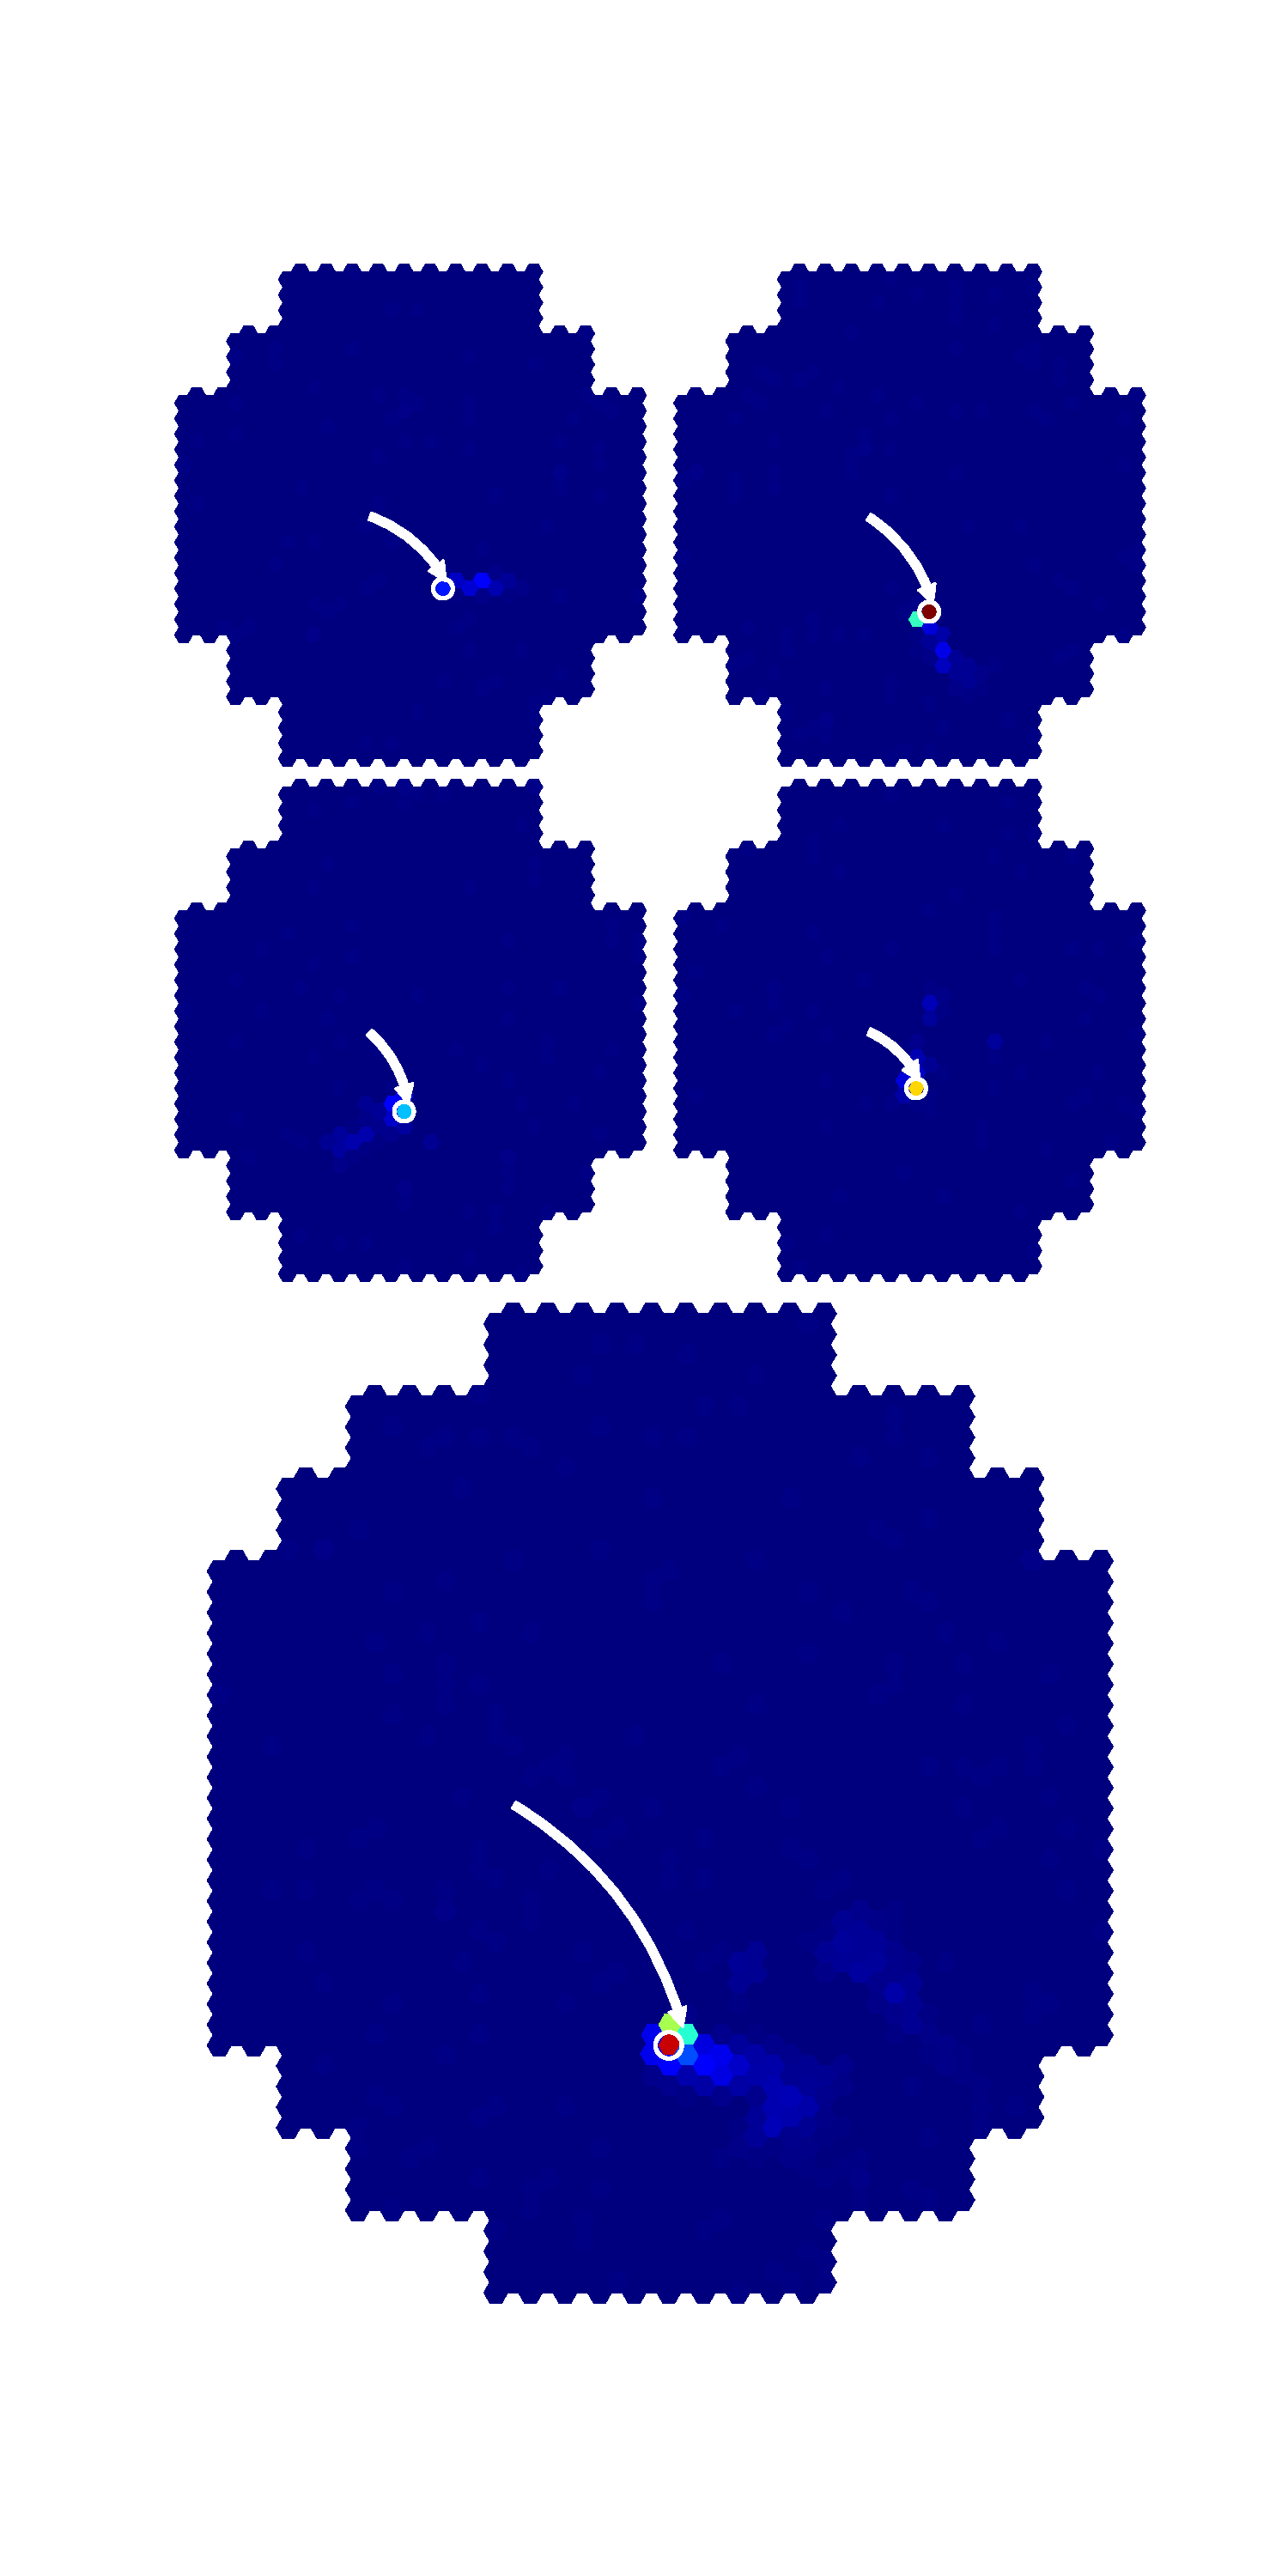
\includegraphics[trim=80 120 80 150,clip,width=\textwidth]{graphDC}
\caption{A typical camera image without the EAS shower. The DC light is visible in every telescope, indicated by the yellow arrow. The shower direction is represented by the white circle. The largest telescope is CT5, but the relative image sizes are not done to scale}
\label{fig:DCtelimage}
\end{minipage}\hfill
\begin{minipage}{0.45\textwidth}
\centering
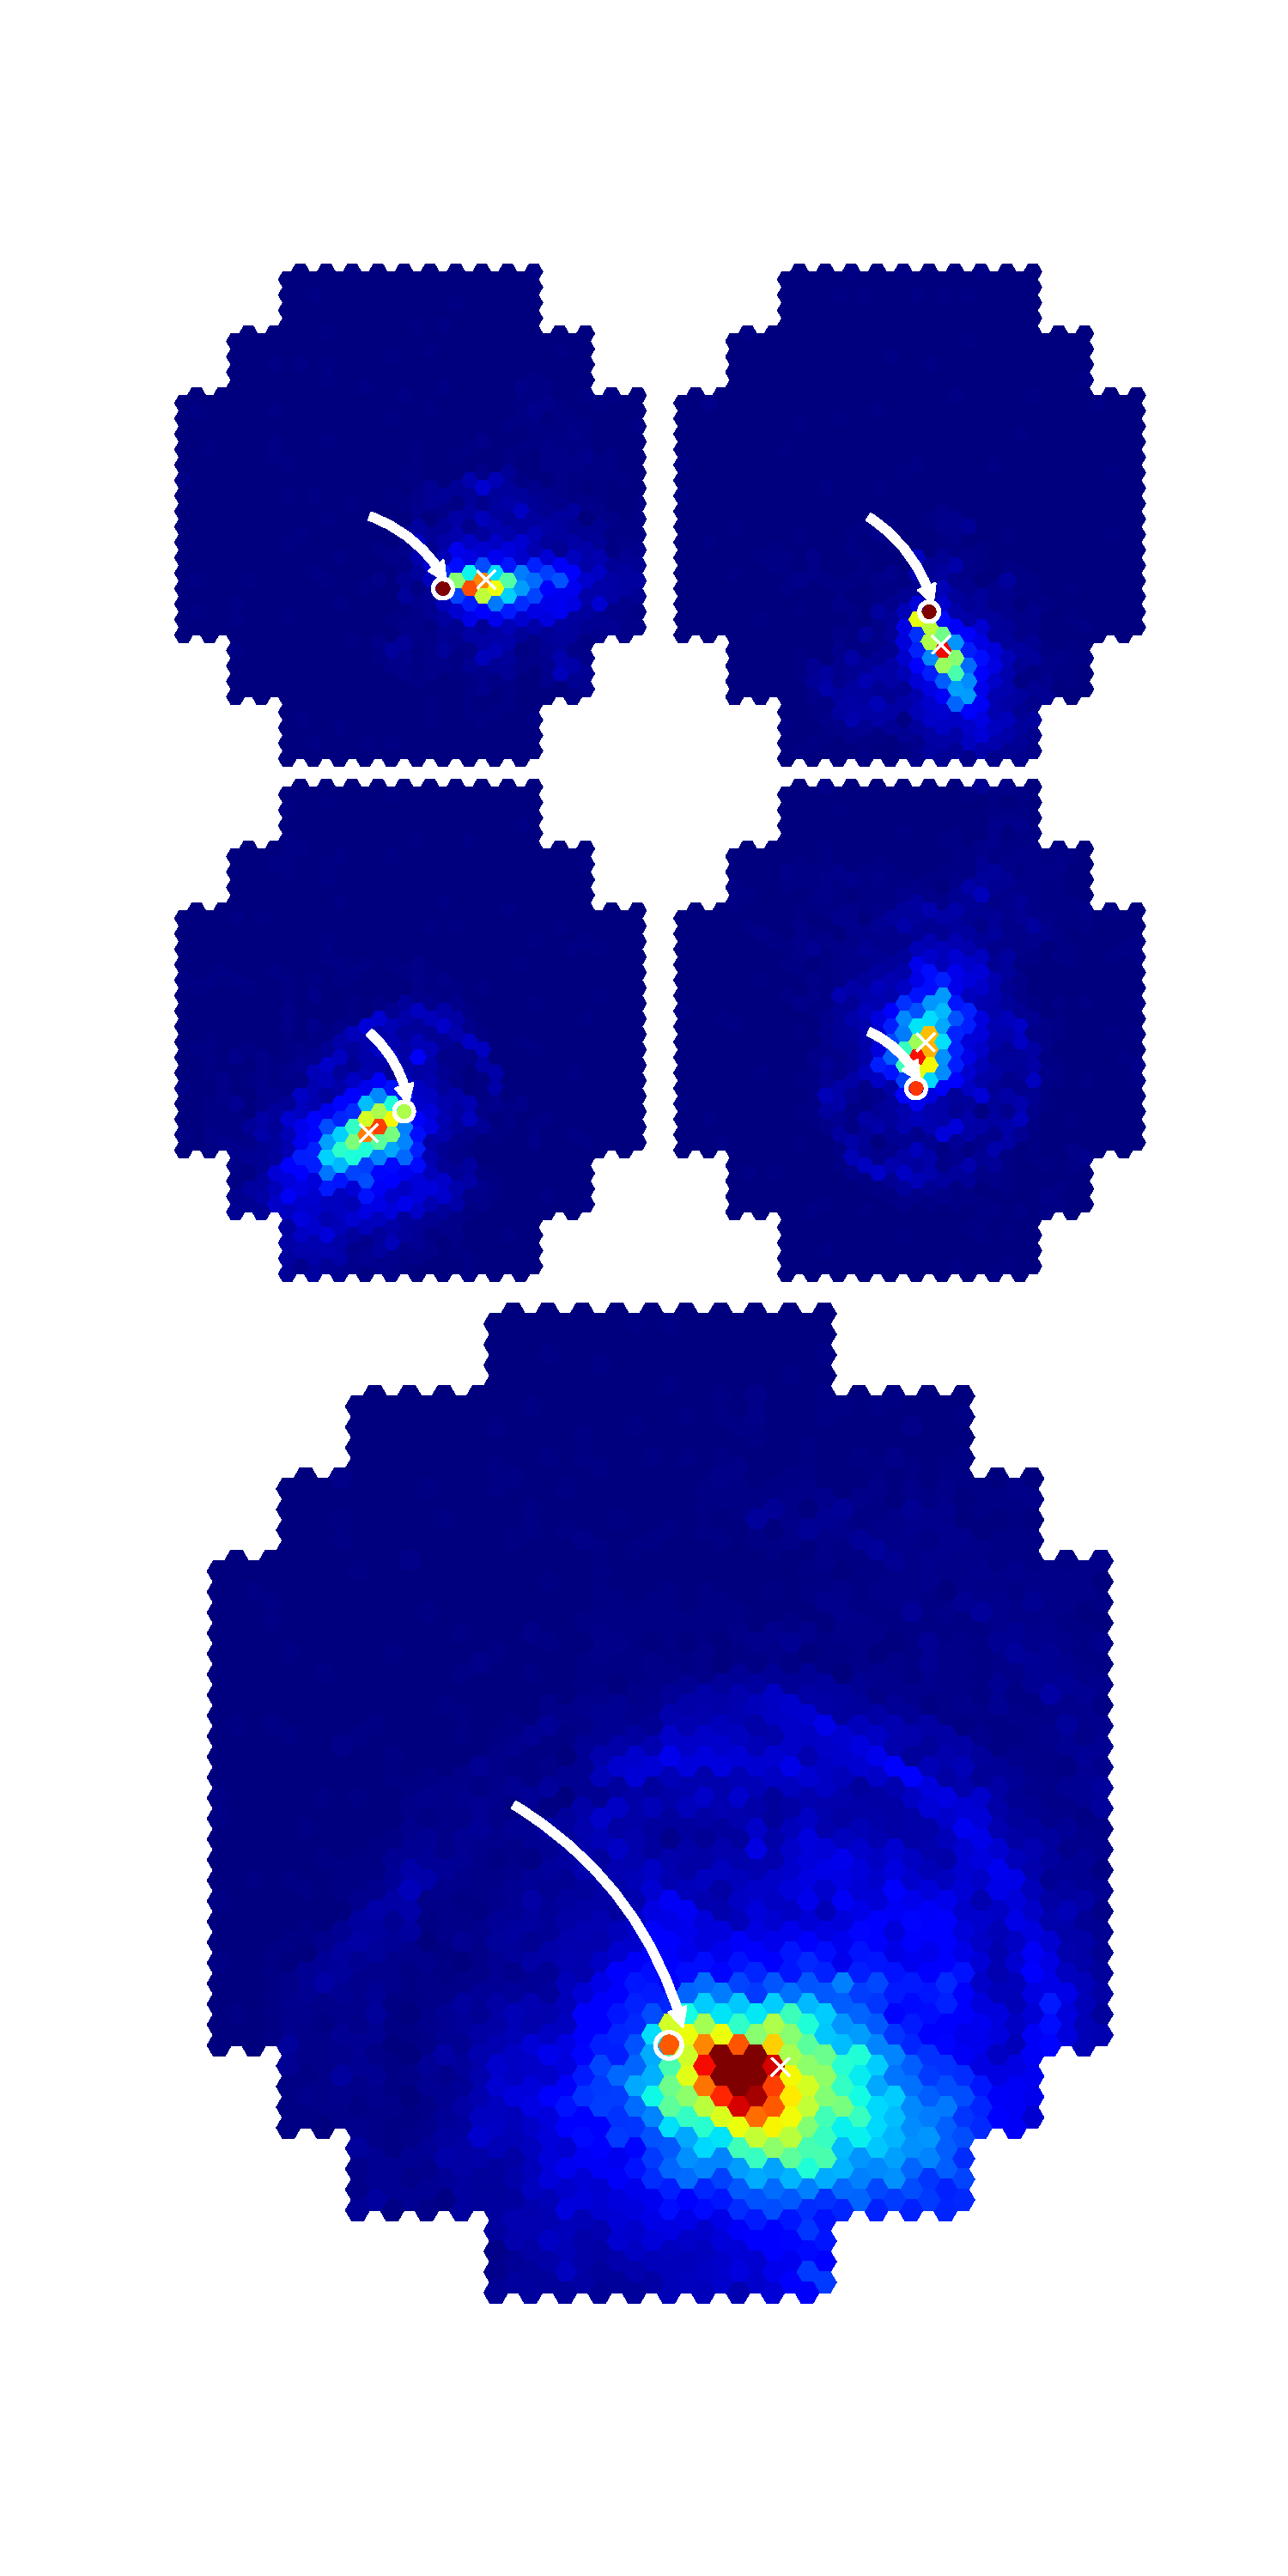
\includegraphics[trim=80 120 80 150,clip,width=\textwidth]{graphfull}
\caption{The same shower as in \ref{fig:DCtelimage} is shown here with the inclusion of the EAS shower. The DC light is pixels are again denoted by an orange circle. The white star represents the BDT-selected DC pixel, while the white cross represents the shower center of gravity.}
\label{fig:cutdistribution2}
\end{minipage}
\restoregeometry
\end{figure}

The HESS telescope has both a high gain Channel 0 and a low gain Channel 1. The Sim\textunderscore telarray value of SOMETHING? for each channel were recorded. The pedestal and gain for each channel were also recorded, and from this, Intensity in the pixel channel was found.

\[ Intensity = (Count - Pedestal)\times Gain \]

In the case of many iron core events, Channel 0 will reach its maximum value and become saturated. Thus Channel 0 ceases to be useful for discriminating between high energy DC and non-DC pixels. Consequently, Channel 0 Intensities were neglected while Channel 1 Intensities were used in all later analysis. This variable $Intensity$ will henceforth be used referred to Channel 1 Intensity.

The Sim\textunderscore telarray package derives various Hillas whole-image parameters. These include the image width and length measured in degrees, from which the aspect ratio $A.R = \frac{width}{length}$ was calculated. The reconstructed shower direction and the shower center of gravity were also calculated, as positions in azimuth and zenith. Additionally the estimated energy and distance from each telescope to core, $r_{core}$,  were recorded.

For every pixel, in addition to the $Intensity$, its location within the telescope image was determined from a standard HESS layout. The variables $ \Delta_{C.o.G}$, $\Delta_{Direction}$ and $\Delta_{Line}$ were defined as the distance from the pixel to the shower center of gravity, shower direction, and the line joining those two points. Furthermore, the nearest neigbouring pixel IDs were calculated for every pixel position, enabling the $Intensity$ in each neighbouring pixel to be found. The largest neighbouring intensity $Intensity_{N.N.max}$ was identified, and the ratio $ Q_{DC} = \frac{Intensity_{N.N.max}}{Intensity} $ was derived. In addition, the Nearest Neighbour Mean Intensity was recorded. 

\section{DC Pixel Identification}  
The original method used by the HESS collaboration \cite{hess07} was initially replicated, for which a number of cuts were applied to each image dataset.

\begin{table}[h!]
  \centering
  \caption{Cuts applied to image pixel sets}
  \label{tab:table1}
  \begin{tabular}{ccc}
    \toprule
    Variable & Cut\\
    \midrule
     $ \Delta_{C.o.G}$ & \textgreater 0.17 \\
     $ \Delta_{C.o.G}$ & \textless 0.91 \\
     $\Delta_{Direction}$ & \textless 0.45 \\
     $\Delta_{Line}$ & \textless 0.23 \\
     Aspect Ratio & \textless 0.75 \\
     $Q_{DC}$ & \textless 0.14$ \times \log(\frac{I_{tot}}{161 \times \cos \theta})$ \\
    \bottomrule
  \end{tabular}
\end{table}

From the subset of pixels satisfying these conditions, the remaining pixel with the smallest $Q_{DC}$ was selected as the DC pixel candidate. In the original analysis, an additional cut $r_{core} \textgreater 0.4$ was applied. However, the uncertainty in determining the core position through Hillas Analysis is typically of the order of $\pm 30m$. Consequently, this particular cut was omitted, along with the Impact Parameter cuts. For every image, the total image amplitude $I_{tot}$ was used alongside the zenith angle $\theta$ to determine a unique $Q_{DC}$ cut. 

The candidates were checked against the true DC pixels from the hadron-only image. Out of 400 events, it was fount that only 55\% of the hadron-free events contained a clear DC signal, as defined by requiring the DC pixel to have $Intensity_{DC} > 150$. This represents a reasonable target number for DC identification. SOMETHING! Of all events, 17\% passed the required cuts. The $Q_{DC}$ was found to be 68\% accurate in identifying the DC pixel in those passing events, as shown in \ref{fig:cutdistribution}. These values served as a benchmark for BDT performance.

\begin{figure}
\begin{center}
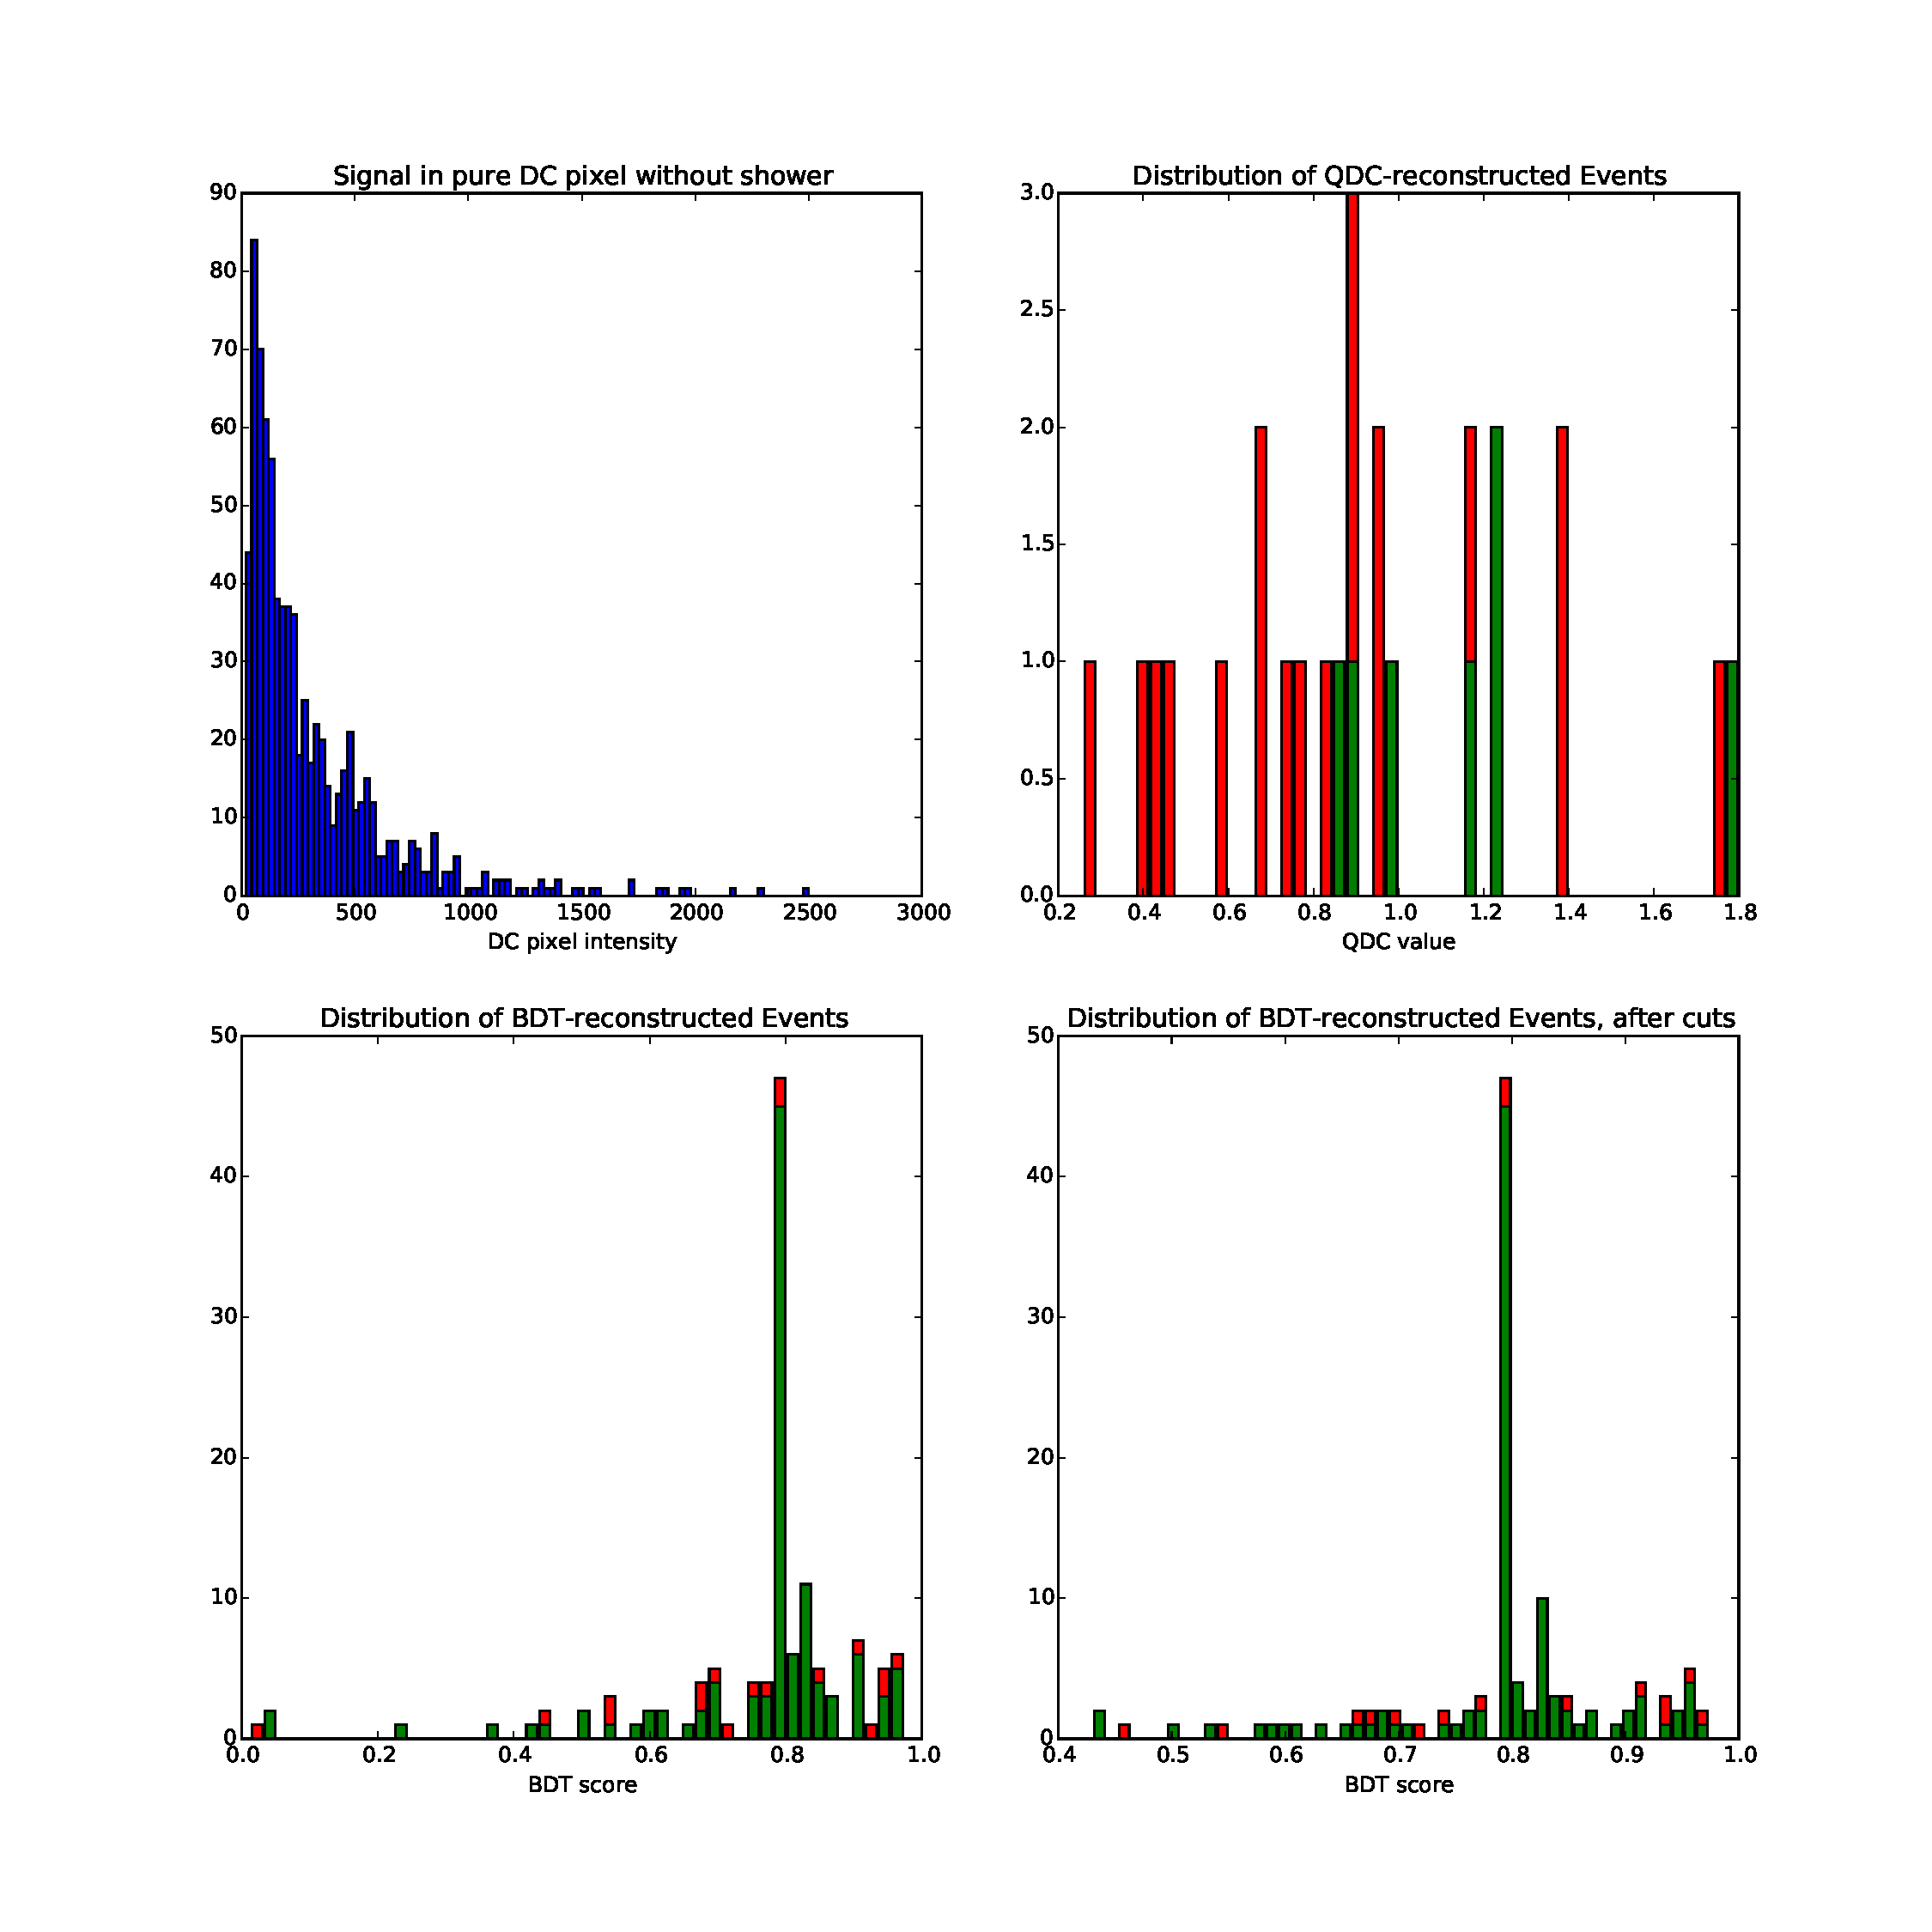
\includegraphics[width=\textwidth]{cutdistribution1None}
\caption{The true $Intensity_{DC}$ in the EAS-free image is shown in the top left, with a broad exponential decay in count as DC intensity increases. Sim\textunderscore telarray requires a minimum of 20 photoelectrons in order for a telescope to be triggered, meaning that only events with a true $Intensity_{DC}>20$ photoelectrons can be studied.  In the top right- the distribution of the dataset is shown, once all $Q_{DC}$ cuts have been applied. In the bottom left, the $P_{signal}$ (BDT score) distribution is shown before any cuts. On the bottom right, we see the same distribution after both $DC_{Count}$ and $P_{signal}$ cuts are applied. All green events are ones in which the DC pixel has been correctly identified, while red events are ones that have been incorrectly identified. We desire both a large number of green events, and a good degree separability of red and green events.}
\label{fig:cutdistribution}
\end{center}
\end{figure} 

For this analysis, a BDT was trained with the Scikit Learn Python package. A set of 2000 simulated events was selected, and randomly split through use of the python random.random() function into two subsets for training and testing. The variable $DC_{Count} = Count-Mean_{N.N}$ was defined as an rough guess of the \textquoteleft DC signal' component in the pixel. Within the subset of training events, every triggered HESS 1 image was used. For each of the 3.6 million triggered image pixels, an entry was formed of the variables listed in table \ref{tab:table2}. A score of 0 was assigned to every pixel to indicate background, with the exception of those that were identified as the true DC pixel through the Shower-Free simulation. These pixels were included with a score of 1, identifying it as a signal pixel. Having created a dataset, the BDT was then trained with a maximum depth of 5, and 100 trees generated.

\begin{table}[h!]
  \centering
  \caption{Relative Feature Importance in BDT training}
  \label{tab:table2}
  \begin{tabular}{ccc}
    \toprule
    Variable & Relative Importance\\
    \midrule
    $DC_{Count}$ & 0.38\\
    $Mean_{N.N}$ & 0.22\\
    $\Delta_{Direction}$ & 0.15\\
    $Q_{DC}$ & 0.11\\
    $raw_{Q}$ & 0.06\\
    $\Delta_{Line}$ & 0.04\\
    $Intensity$ & 0.04\\
    \bottomrule
  \end{tabular}
\end{table}

The relative importance of each \textquoteleft feature' is automatically calculated by the Scikit Learn package, and is also recorded in table \ref{tab:table2}. The variable $DC_{Count}$ was consistently the most importance variable across many combinations of included variables and BDT training parameters. It was found that, under the conditions listed above, the BDT was 99.94 \% accurate for the entire training dataset, and 99.93 \%  accurate for the testing dataset. This indicates that the BDT was not significantly overtrained, which would otherwise be manifested by a large divergence in accuracy between testing and training data.

Having trained the BDT successfully, it was then applied to the same separate dataset as for the classic QDC identification. In each camera image, the event with the largest BDT score was deemed to be \textquoteleft most signal-like', and thus selected as the DC pixel candidate. A cut was applied, requiring $P_{signal} > 0.5$ for the DC candidate to be accepted. A second cut requiring $DC_{Count} > 200$ removed many incorrectly identified events. 

Application of this combined cut greatly increases the successful identification rate. Of the 2000 events, 84\% of events passed all of the required cuts. The BDT was found to be 90 \% accurate in identifying the DC pixel in those passing events. This represents a very significant improvement in DC pixel identification over the previous QDC method, and corresponds to a fivefold increase in the number of HESS data events that can be studied using the LPD method.

HESS2!

\section{Conclusion}
The use of BDT identification has been shown to be superior to the traditional $Q_{DC}$ method, by providing five times as many correctly identified events, once cuts have been applied. Furthermore, the resultant sample has only half the contamination of the $Q_{DC}$ method, with 15\% of the sample being incorrectly identified events rather than 30\% for $Q_{DC}$.

\bibliographystyle{plain}
\bibliography{report}

\end{document}
